\documentclass[../main.tex]{subfiles}
\begin{document}

\begin{definition*}
    给定一个概率空间 $(\Omega,\mathcal F,P)$,若对于某个集合 $T$(称之为\emph{指标集}),$\forall t\in T$,都有一个随机变量 $X_t$,则称 $\{X_t\}_{t\in T}$ 为一个\emph{随机过程}(Stochastic Process),也记作 $\{X_t,t\in T\}$。称 $X_t$ 为该随机过程在 $t$ 时刻的状态,有时也记作 $X(t)$,其取值集合 $S$ 称为\emph{状态空间},即 $\forall t\in T,\forall \omega\in\Omega,X_t(\omega)\in S$。$\forall\omega_0\in\Omega$,称 $\{X_t(\omega_0),t\in T\}$ 为该随机过程的一条\emph{样本轨道}(Sample Path)。
\end{definition*}

随机变量是 $\Omega$ 上的函数,而随机过程是一列随机变量,因此 $X_t(\omega)$ 可以视为 $t,\omega$ 的函数。

\begin{example*}
    设 $X_0,U$ 独立且均服从 $N(0,1)$,令 $X_t=X_0+tU$,则 $\{X_t,t\in\mathbb R\}$ 是一个随机过程,$\forall t\in\mathbb R,X_t\sim N(0,t^2+1)$,如下图所示。
\end{example*}

\begin{figure}[!h]
    \centering
    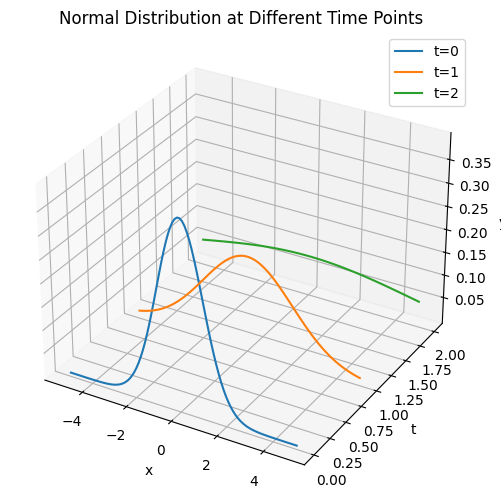
\includegraphics[scale=0.7]{figures/SP_exp1.png}
    \caption*{$\{X_t,t\in\mathbb R\}$ 的分布}
\end{figure}

\begin{example*}
    设 $\{Y_i\}_{i=1}^\infty$ 独立同分布,且 $P(Y_i=1)=P(Y_i=-1)=\frac12$,令 $Y_0=0,X_n=\sum_{i=0}^nY_i$,则 $\{X_n,n\in\mathbb N\}$ 是一个随机过程,属于\emph{随机游走}(Random Walk)。
\end{example*}

如果一个随机过程的 $T$ 是离散的,常称之为\emph{时间序列}(Time Series)。而如果 $S$ 是离散的,有时用\emph{链}(Chain)来称呼这样的随机过程。

\begin{definition*}
    若 $\forall n,\forall t_1<t_2<\cdots<t_n\ (t_1,\cdots,t_n\in T)$,满足 $X_{t_2}-X_{t_1},X_{t_3}-X_{t_2},\cdots,X_{t_n}-X_{t_{n-1}}$ 相互独立,则称 $\{X_t,t\in T\}$ 为\emph{独立增量过程}。若 $T$ 中包含最小指标 $t_0$,则要求 $X_{t_0},X_{t_1}-X_{t_0},X_{t_2}-X_{t_1},\cdots,X_{t_n}-X_{t_{n-1}}$ 相互独立。
\end{definition*}

\begin{definition*}
    若 $\forall t\in T,\forall\tau\text{ s.t. }t+\tau\in T$,满足 $X_{t+\tau}-X_t$ 只依赖 $\tau$(不依赖 $t$),则称 $\{X_t,t\in T\}$ 为\emph{平稳增量过程}。
\end{definition*}

一个随机过程 $\{X_t,t\in T\}$ 是平稳增量过程,等价于 $\forall t_1,t_2\in T,\forall\tau\text{ s.t. }t_i+\tau\in T\ (i=1,2)$,总有 $X_{t_1+\tau}-X_{t_1}$ 与 $X_{t_2+\tau}-X_{t_2}$ 同分布。

\end{document}
